\documentclass[a4paper]{article}
\usepackage[a4paper]{geometry}
\usepackage{amsmath}
\usepackage{amssymb}
\usepackage[utf8]{inputenc}
\usepackage{graphicx}
\usepackage{booktabs}
\usepackage[russian]{babel}
\usepackage{flafter}

\title{Лабораторная работа 2.2.2 \\Измерение теплопроводности воздуха при разных давлениях}
\date{06 марта 2017 г.}
\author{Вячеслав Ждановский, студент 611 группы ФРКТ\\
Шамиль Вагабов, студент 611 группы ФРКТ\\
Станислав Токарев, студент 611 группы ФРКТ}
\begin{document}
	\pagenumbering{gobble}
	\maketitle
	\newpage
	\pagenumbering{arabic}
	\paragraph{Цель работы:}
	измерение перегрева нити при фиксированной мощности нагрева в зависимости от давления воздуха; определение коэффициента теплопроводности при атмосферном давлении, оцена длины свободного пробега, сечения рассеяния и диаметра молекул воздуха; определение области теплопроводности и области теплопередачи (температурного скачка); определение коэффициента аккомодации в области теплопередачи.
	\paragraph{В работе используется:} прибор для определения теплопроводности газа; форвакуумный насос; манометр; вакуумметр; одинарно-двойной мост; реостат; гальванометр; миллиамперметр; источник постоянного напряжения 3-4 В.
	\section{Схема экспериментальной установки}
	\begin{figure}[h!]
		\centering
		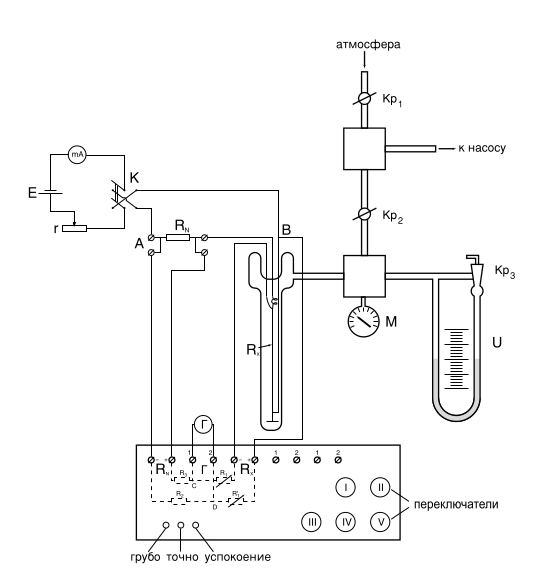
\includegraphics[width=90mm]{pic1.png}
		\caption{Схема установки для измерения теплопроводности воздуха \label{overflow}}
	\end{figure}
	\begin{figure}[h!]
		\centering
		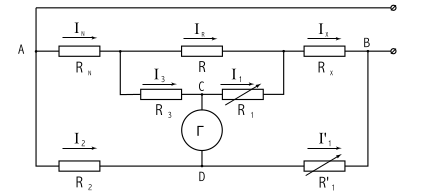
\includegraphics[width=60mm]{pic2.png}
		\caption{Схема установки для измерения теплопроводности воздуха \label{overflow}}
	\end{figure}
	\section{Теоретическая часть}
	Перенос тепла описывается уравнением Фурье:
	\begin{equation}
	q=-\varkappa \cdot \frac{dT}{dx}
	\end{equation}
	где $q$ - плотность теплового потока - количество энергии, переносимой через единичную площадку в единицу времени, $\varkappa$ - коэффициент теплопроводности $\frac{dT}{dx}$ - градиент температуры в направлении $x$. Согласно МКТ коэффициент теплопроводности в газах равен:
	\begin{equation}
	\varkappa=\frac{1}{3}\cdot \lambda \cdot v \cdot n \cdot C^1_v
	\end{equation}
	где $C^1_v$ - теплоемкость в расчете на одну молекулу ($C^1_v=\frac{i}{2}$, $i$ - количество степеней свободы молекулы), $v=\sqrt{\frac{8RT}{\pi \mu}}$ - средняя тепловая скорость молекул, $\lambda$ - длина свободного пробега, а n - концентрация молекул газа. Длина свободного пробега обратно пропорциональна концентрации молекул: 
	$\lambda=\frac{1}{\sqrt{2}\cdot n \cdot \sigma}$; $\sigma$ - сечения рассеяния молекул; $\sigma=\pi d^2$. Поэтому коэффициент теплопроводности газа не зависит от давления.
	Плотность потока тепла в случае сильно разреженного газа (где происходит теплопередача).
	\begin{equation}
	q=\frac{1}{4}\cdot n \cdot v \cdot C^1_v(T_1-T_2)
	\end{equation},
	где $n$ - число молекул, ударяющихся в единицу времени об единичную площадку.
	Сопротивление металлической нити увеличивается при увеличении температуры по закону:
	\begin{equation}
	R=R_0(1 + \alpha t)
	\end{equation}
	где $t$ - температура в $^oC$, $R_0$ - сопротивление при $t=0^oC$.
	Распространение потока тепла $Q$ от горячей нити по радиусу к холодным стенкам:
	\begin{equation}
	Q=-2\pi \cdot r \cdot L \cdot \varkappa \frac{dT}{dr}
	\end{equation}
	где $L$ - высота цилиндра, $2\pi r L$ - площадь цилиндрической поверхности на расстоянии $r$ от нити. После интегрирования по радиусу получаем формулу для разности температур между нитью и стенкой цилиндра:
	\begin{equation}
	T_{r_\text{н}} - T_R=\frac{Q}{2\pi L \varkappa}*\ln\frac{R}{r_\text{н}}
	\end{equation}
	где $Q$ - мощность Джоулева тепла, выделяющегося в нагретой нити, $T_\text{н}$ - температура нити, $T_R$ - температура внутренней стенки цилиндра. 
	При низких давлениях закон Фурье нарушается - это область \textbf{теплопередачи}. Для этой области поток тепла, согласно (3), будет равен:
	\begin{equation}
	Q = 2\pi \cdot r_\text{н} \cdot L \cdot \frac{1}{4}\cdot n \cdot v \cdot C^1_v(T_{r_\text{н}} - T_R)
	\end{equation}
	\begin{equation}
	T_{r_\text{н}} - T_R = \frac{4Q}{2\pi L n v C^1_v r_\text{н}s}
	\end{equation}
	Здесь учтен коэффициент аккомодации $s$, учитывающий, что температуру нити приобретает только часть молекул, сталкивающихся с нитью. Преобразуем выражение, выразив его через $\varkappa = const$ при высоком давлении.
	\begin{equation}
	T_{r_\text{н}} - T_R = \frac{4Q}{2\pi L n v C^1_v r_\text{н}s}=\frac{4\lambda Q}{3r_\text{н}s\cdot 2\pi L \varkappa}
	\end{equation}
	Учет обоих вкладов дает:
	\begin{equation}
	T_{r_\text{н}} - T_R = \frac{Q}{2\pi L \varkappa}\cdot \ln \frac{R}{r_\text{н}}\cdot \left[1-ln\left(1+\frac{\lambda}{r_\text{н}}\right)/\alpha + \frac{4\lambda}{3r_\text{н}s}/\alpha\right]
	\end{equation}
	\section{Ход работы}
	\paragraph*{Параметры установки}
	\begin{equation}
	L=220\pm 2 \text{ мм}
	\end{equation}
	\begin{equation}
	2r = 0,05 \text{ мм}
	\end{equation}
	\begin{equation}
	2R = 10 \text{ мм}
	\end{equation}
	\begin{equation}
	\rho_\text{ масла}=0,885 \text{г/см}^3
	\end{equation}
	\begin{equation}
	T=295 K, P_0=746,2 \text{ торр}
	\end{equation}
	\begin{equation}
	\alpha=3,83\cdot 10^{-3} \text{ }^oC^{-1}
	\end{equation}
	1. Ознакомимся со схемами установки. \\
	2. Включим приборы, впустим воздух в установку. \\
	3. Снимем зависимость напряжения $U$ от величины тока $I$.
	\begin{table}[h!]
 		\centering
    	\begin{tabular}{| c | c | c | c |}
    		\hline
    		I, мА & U, мВ & Q, $10^{-6}$ Вт & R, Ом \\
    		\hline
    		70,744 &	889,2 &	62905,56	&12,56926 \\
    		\hline
66,573 & 825,3 & 	54942,7 & 	12,39692 \\
    		\hline
59,36 & 	722,63 & 	42895,32 & 	12,17369 \\
    		\hline
50,927	 & 607,9	 & 30958,52	 & 11,93669 \\
    		\hline
45,461	 & 537,4	 & 24430,74	 & 11,82112 \\
    		\hline
39,473	 & 462,29	 & 18247,97	 & 11,71155 \\
    		\hline
31,202	 & 361,79	 & 11288,57	 & 11,59509 \\
    		\hline
26,772	 & 309,12	 & 8275,761	 & 11,54639 \\
    		\hline
    	\end{tabular}
	\end{table}
	4.Используя (4), найдем сопротивление при комнатной температуре $R_0 = 11.36 \text{ Ом}$
	5. Произведем аналогичные измерения при разных давлениях и построим график зависимости $t(Q)$
	\begin{table}[h!]
 		\centering
    	\begin{tabular}{| c | c | c | c |}
    		\hline
    		I, мА & U, мВ & Q, $10^{-6}$ Вт & R, Ом \\
    		\hline
    		71,845 & 873,17	 & 62732,9 & 	12,15352 \\
    		\hline
65,345	 & 785,15	 & 51305,63 & 	12,01546\\
    		\hline
55,196	 & 653,38	 & 36063,96 & 	11,83745\\
    		\hline
43,707	 & 510,27	 & 22302,37	 & 11,67479\\
    		\hline
36,126	 & 418,9	 & 15133,18 & 	11,59553\\
    		\hline
30,77	 & 355,55	 & 10940,27 & 	11,55509\\
    		\hline
26,785	 & 309,06	 & 8278,172 & 	11,53855\\
    		\hline
    	\end{tabular}
    	\caption{P=95,403 Па}
	\end{table}
	\begin{table}[h!]
 		\centering
    	\begin{tabular}{| c | c | c | c |}
    		\hline
    		I, мА & U, мВ & Q, $10^{-6}$ Вт & R, Ом \\
    		\hline
    		72,46 & 879,95	 & 63761,18	 & 12,14394 \\
    		\hline
65,798	 & 791,55	 & 52082,41	 & 12,03\\
    		\hline
58,55	 & 697,81	 & 40856,78	 & 11,91819\\
    		\hline
43,845	 & 514,75 & 	22569,21 & 	11,74022\\
    		\hline
36,209	 & 422,51	 & 15298,66	 & 11,66865\\
    		\hline
30,825 & 	358,4 & 	11047,68 & 	11,62693\\
    		\hline
26,826 &	311,225	 & 8348,922	& 11,60162 \\ 
    		\hline
    	\end{tabular}
    	\caption{P=130,095 Па}
	\end{table}
	\begin{table}[h!]
 		\centering
    	\begin{tabular}{| c | c | c | c |}
    		\hline
    		I, мА & U, мВ & Q, $10^{-6}$ Вт & R, Ом \\
    		\hline
    		72,615 &	877,533 &	63722,06 &	12,08473\\
			\hline
60,276&	717,91	&43272,74&	11,91038 \\
			\hline
43,85	&514,61	&22565,65	&11,73569\\
			\hline
36,202&	422,7	&15302,59	&11,67615\\
			\hline
30,817	&358,73	&11054,98&	11,64065\\
			\hline
26,817&	311,57&	8355,373&	11,61838\\
			\hline
23,737	&275,43	&6537,882&	11,6034\\
			\hline
    	\end{tabular}
    	\caption{P=225,498 Па}
	\end{table}
	\begin{table}[h!]
 		\centering
    	\begin{tabular}{| c | c | c | c |}
    		\hline
    		I, мА & U, мВ & Q, $10^{-6}$ Вт & R, Ом \\
    		\hline
    		72,865	& 872,36 &	63564,51	&11,97228\\
    		\hline
64,017	&761,03	&48718,86	&11,88794\\
    		\hline
43,84&	514,436	&22552,87&	11,7344\\
    		\hline
36,186	&423,07	&15309,21&	11,69154\\
    		\hline
30,799&	359,313	&11066,48	&11,66639\\
    		\hline
26,802	&312,246&	8368,817&	11,6501\\
    		\hline
23,725&	276,14	&6551,422	&11,6392\\
    		\hline
    	\end{tabular}
    	\caption{P=780,57 Па}
	\end{table}
	\begin{table}[h!]
 		\centering
    	\begin{tabular}{| c | c | c | c |}
    		\hline
    		I, мА & U, мВ & Q, $10^{-6}$ Вт & R, Ом \\
    		\hline
    		72,789 &	873,63	& 63590,65 &	12,00223\\
    		\hline
63,985	& 761,8	& 48743,77	& 11,90592\\
    		\hline
55,52& 	656,68	& 36458,87 &	11,82781\\
    		\hline
43,83	& 514,52	& 22551,41& 	11,73899\\
    		\hline
36,182	& 493,026& 	17838,67& 	13,62628\\
    		\hline
26,8	& 312,125	& 8364,95	&11,64646\\
    		\hline
23,722	&275,993	&6547,106	&11,63447\\
    		\hline
    	\end{tabular}
    	\caption{P=745,878 Па}
	\end{table}
	\begin{table}[h!]
 		\centering
    	\begin{tabular}{| c | c | c | c |}
    		\hline
    		I, мА & U, мВ & Q, $10^{-6}$ Вт & R, Ом \\
    		\hline
    		72,763	& 874,2	& 63609,41& 	12,01435\\
    		\hline
63,975	& 762,13	& 48757,27	& 11,91293\\
    		\hline
58,632	& 695,265	& 40764,78	& 11,85812\\
    		\hline
45,776	& 537,755	& 24616,27	& 11,74753\\
    		\hline
37,504	& 438,5	& 16445,5	& 11,69209\\
    		\hline
31,752	& 370,23& 	11755,54& 	11,66005\\
    		\hline
27,522	& 320,352	& 8816,728	& 11,63985\\
    		\hline
    	\end{tabular}
    	\caption{P=581,091 Па}
	\end{table}
	\begin{table}[]
 		\centering
    	\begin{tabular}{| c | c | c | c |}
    		\hline
    		I, мА & U, мВ & Q, $10^{-6}$ Вт & R, Ом \\
    		\hline
    		72,675 &	875,26&	63609,52&	12,04348\\
    		\hline
60,275	&716,73	&43200,9	&11,891\\
    		\hline
55,501&	657,22	&36476,37	&11,84159\\
    		\hline
43,837	&514,6	&22558,52&	11,73894\\
    		\hline
36,191	&422,895	&15304,99&	11,68509\\
    		\hline
30,806	&359,009	&11059,63&	11,65387\\
    		\hline
26,808	&311,885	&8361,013	&11,63403\\
    		\hline
    	\end{tabular}
    	\caption{P=312,228 Па}
	\end{table}
	\\6. Построим зависимость $t$ от $Q$.
	\\7. Построим зависимость $t$ от $\frac{1}{P}$ и найдем из него $\varkappa=2,53\cdot10^{-2} \frac{B}{\text{м}\cdot K}$.
	\begin{table}
 		\centering
    	\begin{tabular}{| c | c |}
    		\hline
    		t, K & Q, $10^{-6}$ Вт\\
    		\hline
    		27,79355 & 62905,56\\
    		\hline
23,83237&	54942,7\\
    		\hline
18,70164	&42895,32\\
    		\hline
13,25465&	30958,52\\
    		\hline
10,59835&24430,74\\
    		\hline
8,079967	&18247,97\\
    		\hline
5,403276&	11288,57\\
    		\hline
4,284001	&8275,761\\
    		\hline
18,23826&	62732,9\\
    		\hline
15,06492	&51305,63\\
    		\hline
10,97369&	36063,96\\
    		\hline
7,235064&	22302,37\\
    		\hline
5,413313	&15133,18\\
    		\hline
4,483831&	10940,27\\
    		\hline
4,103715&	8278,172\\
    		\hline
18,018	&63761,18\\
    		\hline
15,3992	&52082,41\\
    		\hline
12,82935&	40856,78\\
    		\hline
8,73895	&22569,21\\
    		\hline
7,093873	&15298,66\\
    		\hline
6,134993	&11047,68\\
    		\hline
5,55331	&8348,922\\
    		\hline
16,65719&	63722,06\\
    		\hline
12,64983	&43272,74\\
    		\hline
8,634802	&22565,65\\
    		\hline
7,266357	&15302,59\\
    		\hline
6,450486&	11054,98\\
    		\hline
5,938486	&8355,373\\
    		\hline
5,594362	&6537,882\\
    		\hline
14,0725	&63564,51\\
    		\hline
12,13401&	48718,86\\
    		\hline
8,605105&	22552,87\\
    		\hline
7,620025&	15309,21\\
    		\hline
7,041915&	11066,48\\
    		\hline
6,667634&	8368,817\\
    		\hline
6,417073&	6551,422\\
    		\hline
14,76082&	63590,65\\
    		\hline
12,54724&	48743,77\\
    		\hline
10,75207&	36458,87\\
    		\hline
8,710687&	22551,41\\
    		\hline
52,08781&	17838,67\\
    		\hline
6,583846&	8364,95\\
    		\hline
6,308478	&6547,106\\
    		\hline
15,03944&	63609,41\\
    		\hline
12,70857&	48757,27\\
    		\hline
11,4486&	40764,78\\
    		\hline
8,906967&	24616,27\\
    		\hline
7,632621&	16445,5\\
    		\hline
6,896373&	11755,54\\
    		\hline
6,432072&	8816,728\\
    		\hline
15,70903&	63609,52\\
    		\hline
12,20442	&43200,9\\
    		\hline
11,06876&	36476,37\\
    		\hline
8,709548	&22558,52\\
    		\hline
7,471763&	15304,99\\
    		\hline
6,754177&	11059,63\\
    		\hline
6,298201&	8361,013\\
    		\hline
    	\end{tabular}
    	\caption{Зависимость t от Q}
	\end{table}
	
	\section{Контрольные вопросы}
	1. Основное изменение температуры происходит в области прилежащей к нити, практически - на расстояниях порядка нескольких её радиусов. Поэтому наиболее резкие изменения характера процесса теплопроводности лежат в том диапазоне давлений, когда длина свободного пробега молекул газа приближается к радиусу нити.
	2. Молекулы, отстоящие от стенки больше чем на несколько лямбд (длин свободного пробега молекул), с ней не соударяются и сталкиваются только между собой. Теплопередача на таких расстояниях ничем не отличается от теплопередачи в ещё более удаленных от стенки областях и подчиняется закону Фурье (лабник стр 119 формула (1) ). Поэтому можно ожидать, что величина температурного скачака будет пропорциональна ширине аномальной области, т.е. лямбде,и,следовательно, обратно пропорциональна давлению P

	\begin{figure}[htb!]
		\centering
		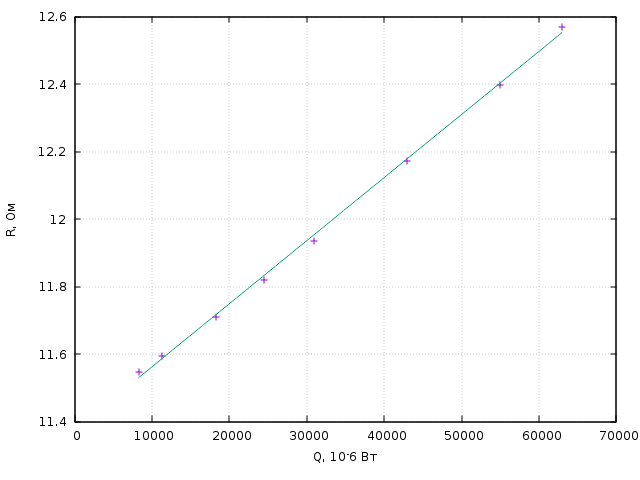
\includegraphics[width=100mm]{plot1.png}
		\caption{Зависимость R от Q\label{overflow}}
	\end{figure}
	\begin{figure}[htb!]
		\centering
		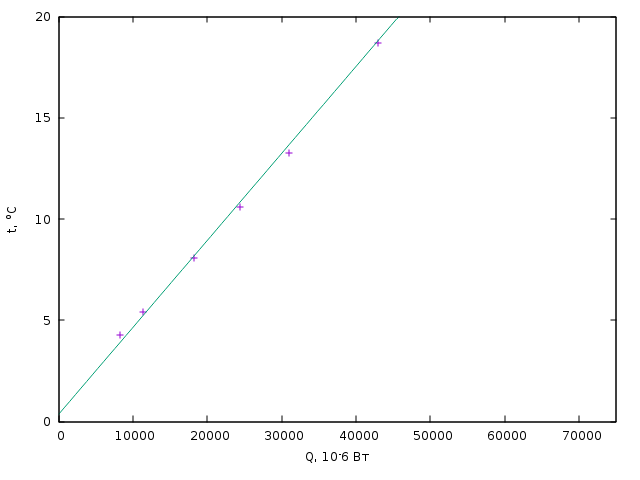
\includegraphics[width=100mm]{plot2.png}
		\caption{Зависимость t от Q для первых трех давлений\label{overflow}}
	\end{figure}
	\begin{figure}[htb!]
		\centering
		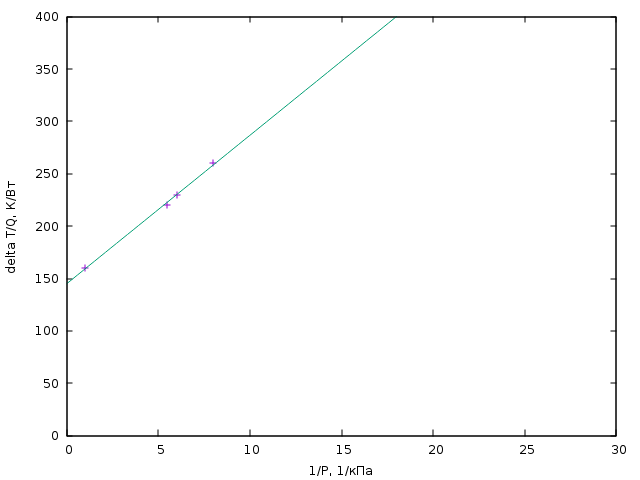
\includegraphics[width=100mm]{plot3.png}
		\caption{Зависимость температуры нити от давления воздуха\label{overflow}}
	\end{figure}
\end{document}